\documentclass{report}
\usepackage[utf8]{inputenc}

\usepackage{graphicx}

% Margins
\usepackage[left=2.5cm, right=2.5cm, bottom=2.5cm]{geometry}

% Example
\usepackage{amsthm}
\theoremstyle{plain}
\newtheorem{example}{Example}[section]

% Default no indent
\setlength\parindent{0pt}

\begin{document}

\begin{titlepage}

\includegraphics[width=0.35\textwidth]{logo-politecnica.png}

\vspace{3\baselineskip}

\begin{center}
\fontsize{30pt}{30pt}\selectfont \textbf{Snowman Editor} \\ 
\huge A level design tool for the game A Good Snowman Is Hard To Build

\vspace{1\baselineskip}

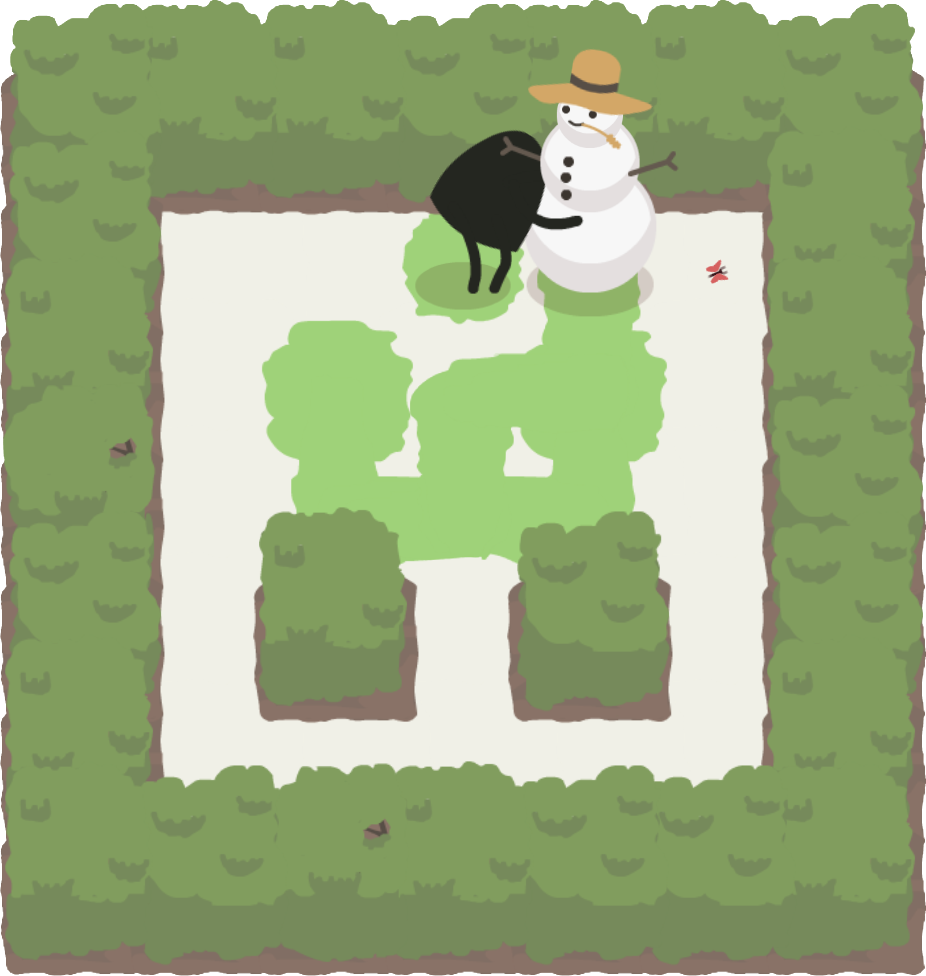
\includegraphics[width=0.5\textwidth]{game-image-2.png}
\vspace*{\fill}

\end{center}

\begin{description}
    \item[Study:] Grau en Enginyeria Informàtica
    \item[Document:] Summary
    \item[Author:] Gerard Martin Teixidor
    \item[Email:] gerardmartinteixidor@gmail.com
    \item[Director:] Gustavo Ariel Patow and Mateu Villaret Auselle
    \item[Department:] Informàtica, Matemàtica Aplicada i Estadística (IMAE)
    \item[Area:] Llenguatges i Sistemes Informàtics (LSI)
    \item[Call:] September/2018
\end{description}
\end{titlepage}

\chapter{Introduction}
In the design of video-games, one of the most important aspects to consider is the difficulty in the design of the different levels. A common problem is the possibility of finding possible solutions that were not planned. These solutions may not be desired because they can break the game dynamics. Hence, it is introduced the idea to create a tool to facilitate the design of those levels by detecting unwanted solutions.

This problem can be seen as a Planning problem, since, given the game state and the possible actions the player can perform, the solutions a level may have can be searched. Once the solutions are found, those that were not considered in the original design can be removed.

Usually this unwanted solutions are shorter, therefore easier solutions, than the designed solution. One of the goals of this project is, given a level, find the optimal solution, which will allow to check if there exist any solution easier than the designed one. Finding an optimal solution is not a simple task since exploring a game search tree by uninformed algorithms can be impossible in a reasonable time. Hence, one part of this project will be focused on reducing this previously described problem to Satisfiability Modulo Theories (\emph{SMT}).

Since finding the optimal is a hard problem, in this project, two different problem relaxations will be presented which will allow to solve the problem in a plausible time.

\section{Personal motivations}
I had chosen this project because it merges the two worlds which I am more passionate about, video-games and optimization. Furthermore, is also a great way to go in depth about AI, since Planning is a well known branch of this topic.

This project has was not easy, despite this I enjoyed working on it and spending much free time on it. 

\section{Project objectives}
The main objectives of this project is the development of this tool for a concrete game, \emph{A Good Snowman is Hard to Build}. This tool, named \emph{Snowman Editor}, will consist of the following parts:
\begin{itemize}
    \item Solve a given level, with an heuristic approach, using the Planning Domain Definition Language (\emph{PDDL}) and multiple solvers
    \item Solve a given level, with an optimal approach, using Satisfiability Modulo Theories (\emph{SMT}) 
    \item A graphical level editor
\end{itemize}

\section{A Good Snowman is Hard to Build}
\emph{A Good Snowman is Hard to Build} is a commercial game based on the popular Sokoban transport puzzle. The goal is to build a snowman from tree balls, each one smaller than the other. 

\begin{center}
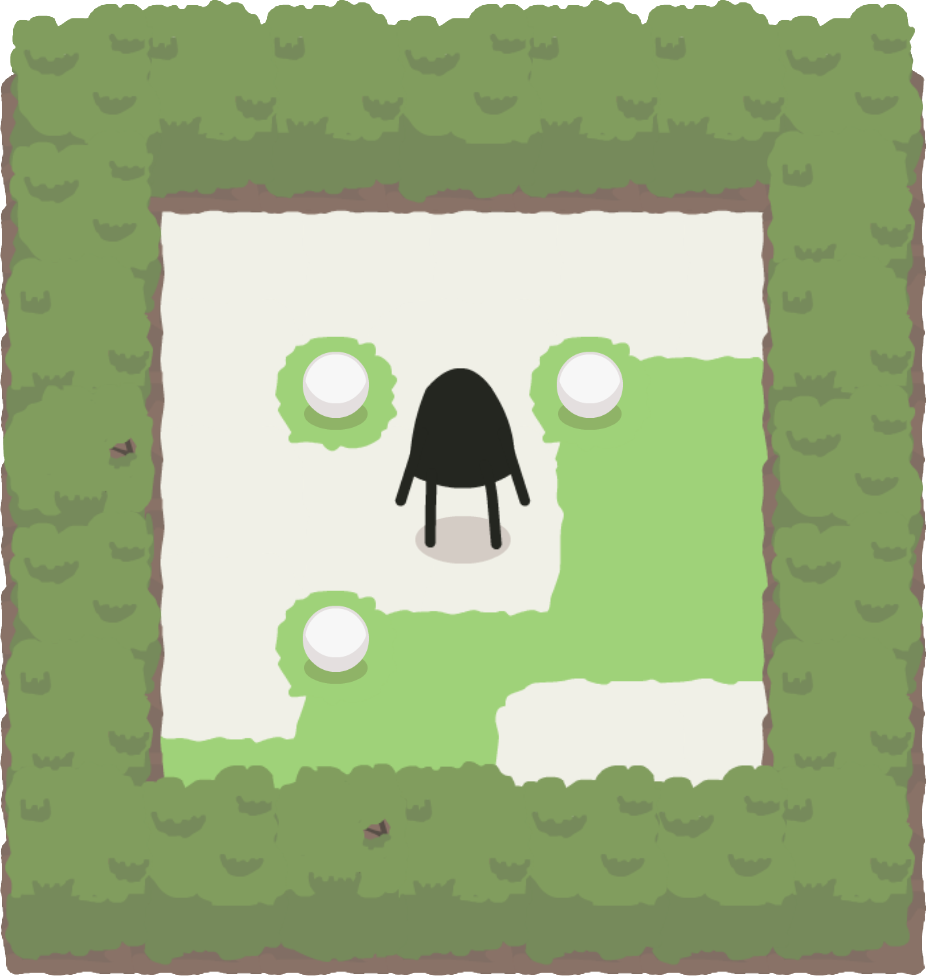
\includegraphics[width=0.2\textwidth]{andy-1.png}
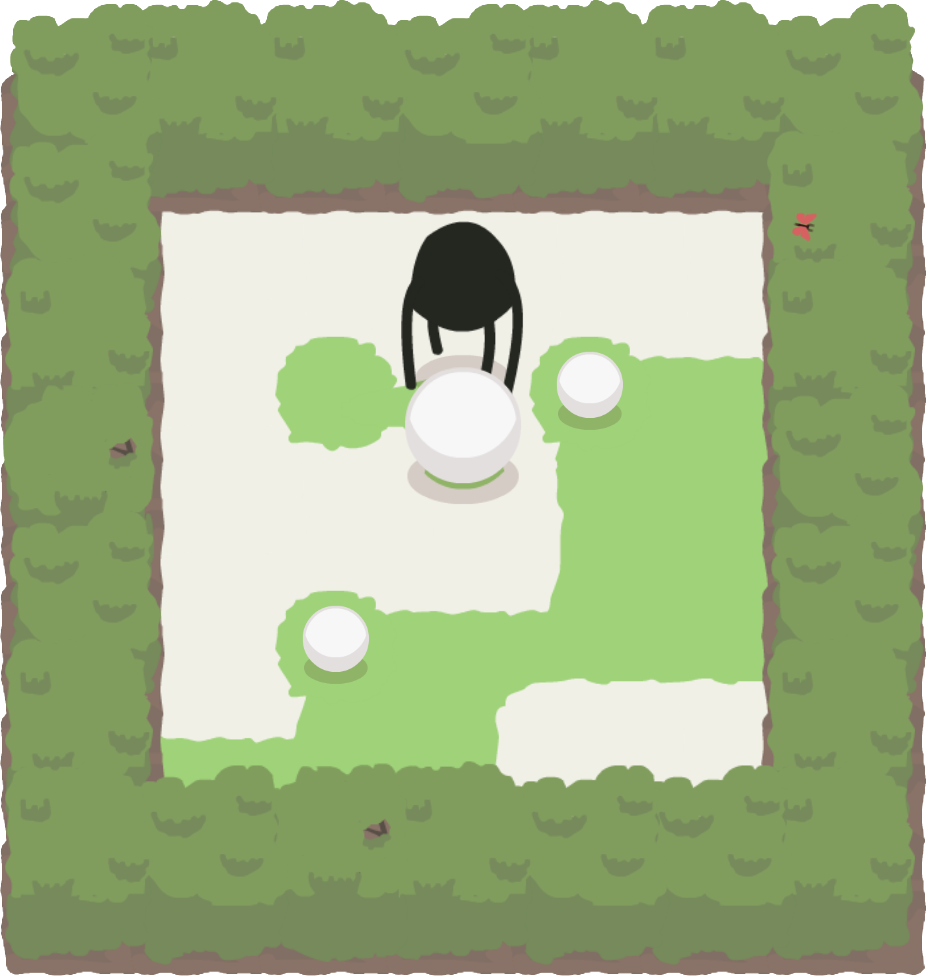
\includegraphics[width=0.2\textwidth]{andy-2.png}
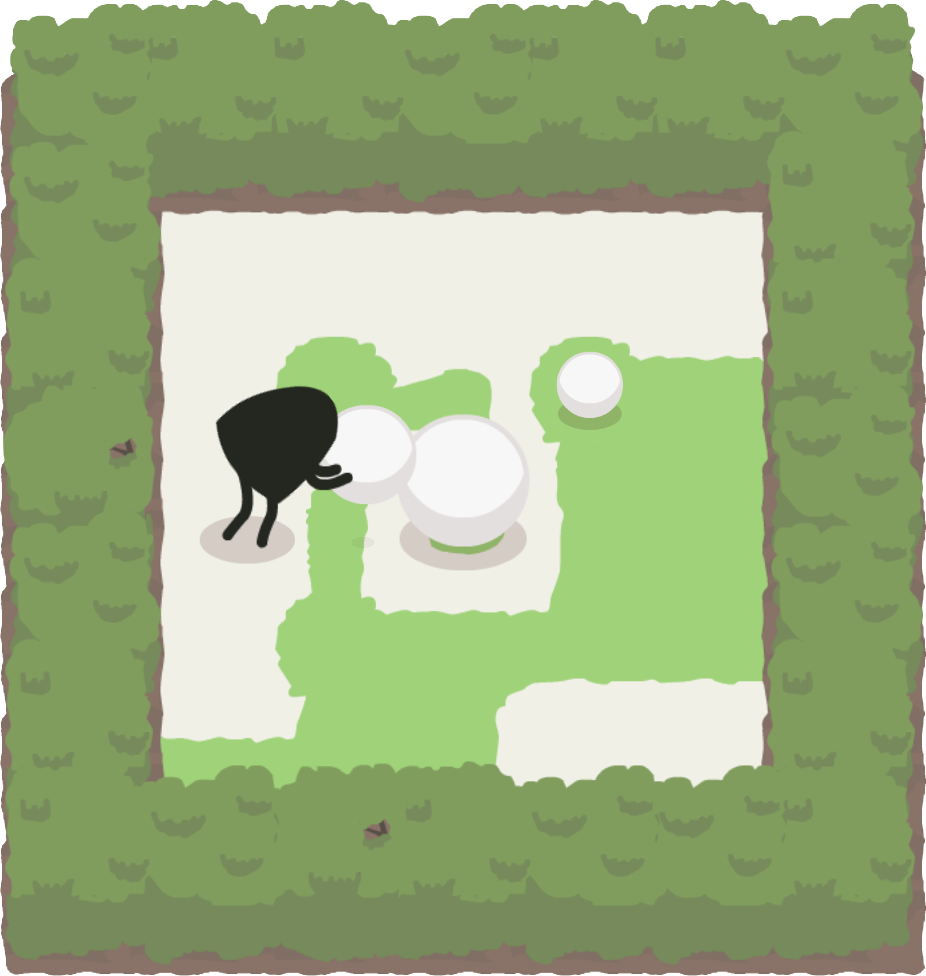
\includegraphics[width=0.2\textwidth]{andy-3.png}
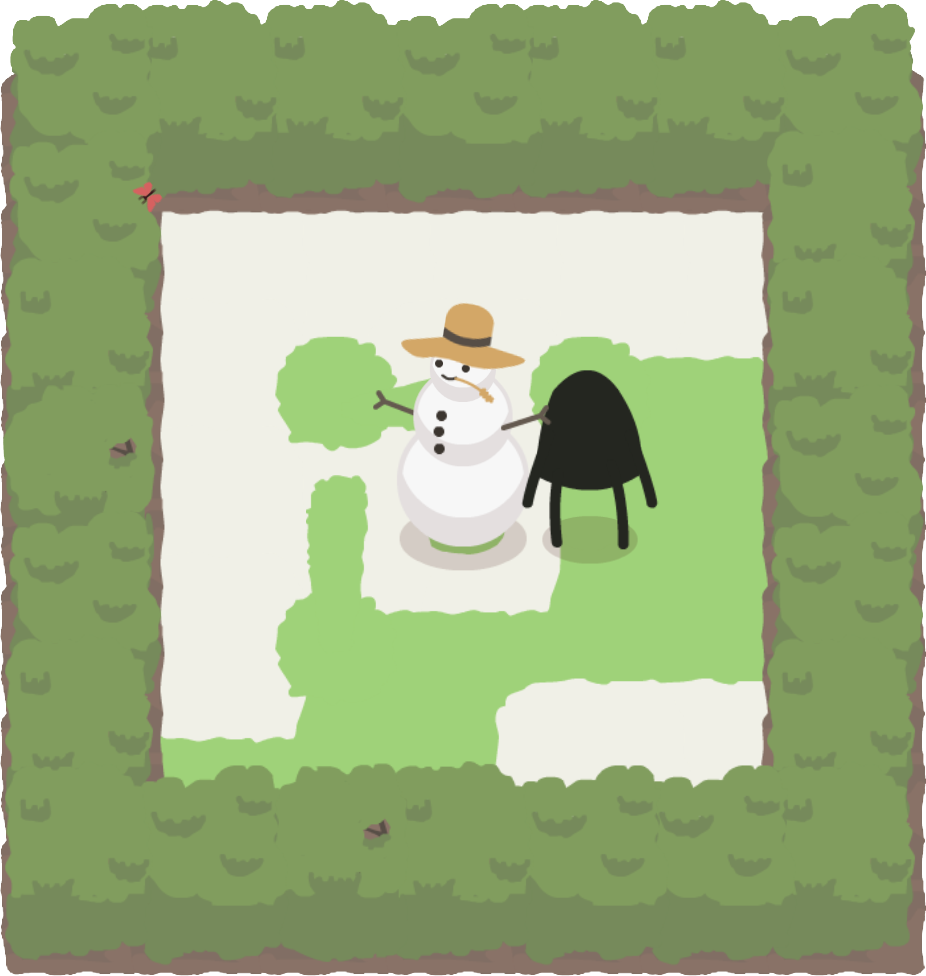
\includegraphics[width=0.2\textwidth]{andy-4.png}
\end{center}

The game consists of multiple levels arranged in an open world layout. For this project each individual level will be seen as a different problem instance. A complete instance solution can be found in the Example~\ref{ex:complete-solution}.

\subsection{Game mechanics}
The game has two worlds with different mechanics each one. This project is focused on the  ``real world`` mechanics but, with minor changes, it should be easy to adapt it to the ``dream world`` mechanics.
The rules describing the ``real world`` mechanics are the following:
\begin{enumerate}
\item The character can only push the balls from behind. 
\item The character can also push and pop a ball over other balls.
\item A ball can not be pop from a ball to directly be on top of another ball.
\item The ball below must be larger.
\item Each ball can have three sizes: small, medium and large.
\item When the ball is rolled on top of snow on the floor it increases its size by one unit, and removes the snow on the floor.
\item When rolled, a large ball does not increase its size though it also removes the snow.
\item Balls can only grow.
\item A level can have multiple snowmans. The number of balls in a level has to be a multiple of three and bigger than 0.
\item Once the snowman is built, you can not pop the top ball. This rule currently is not implemented in the SMT approach. % IMPLMENET
\item A snowman is formed by three balls.
\item A snowman can be built anywhere.
\end{enumerate}

\newcommand{\andyWidth}{0.2}

\newpage

\begin{example}
\label{ex:complete-solution}
A complete solution to the Andy level:
\begin{center}
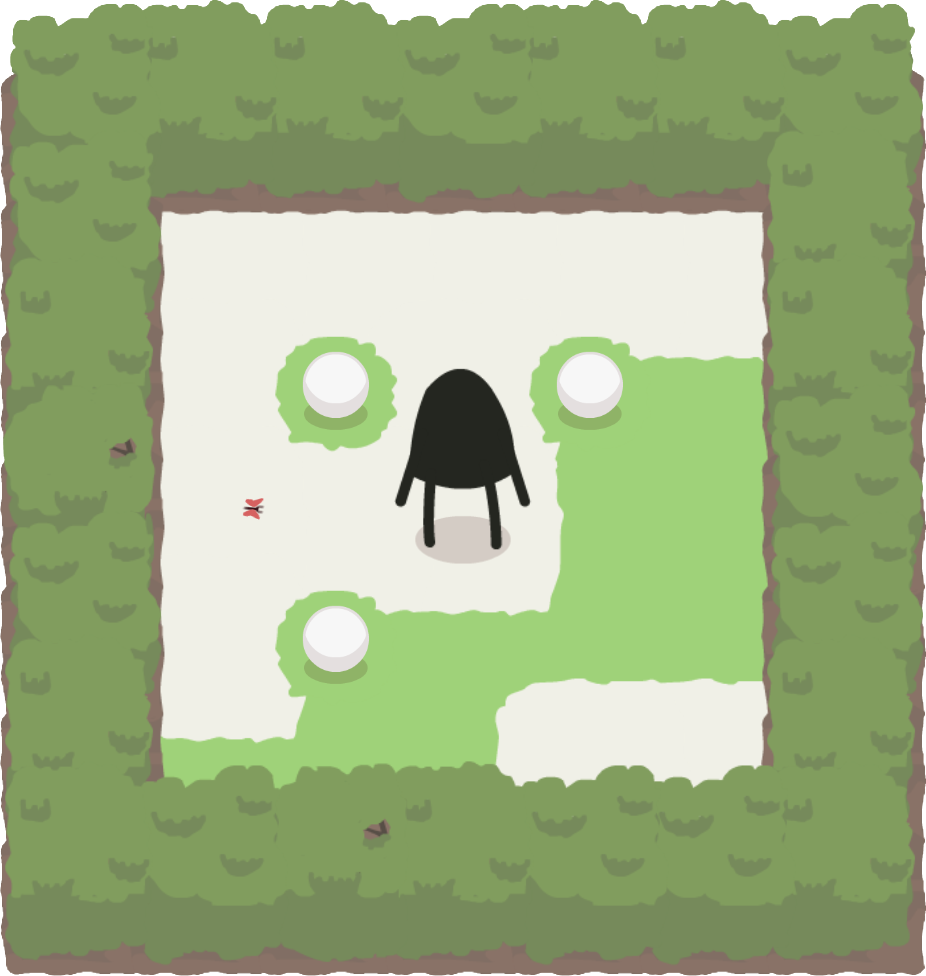
\includegraphics[width=\andyWidth\textwidth]{andy-basic-1.png} \quad
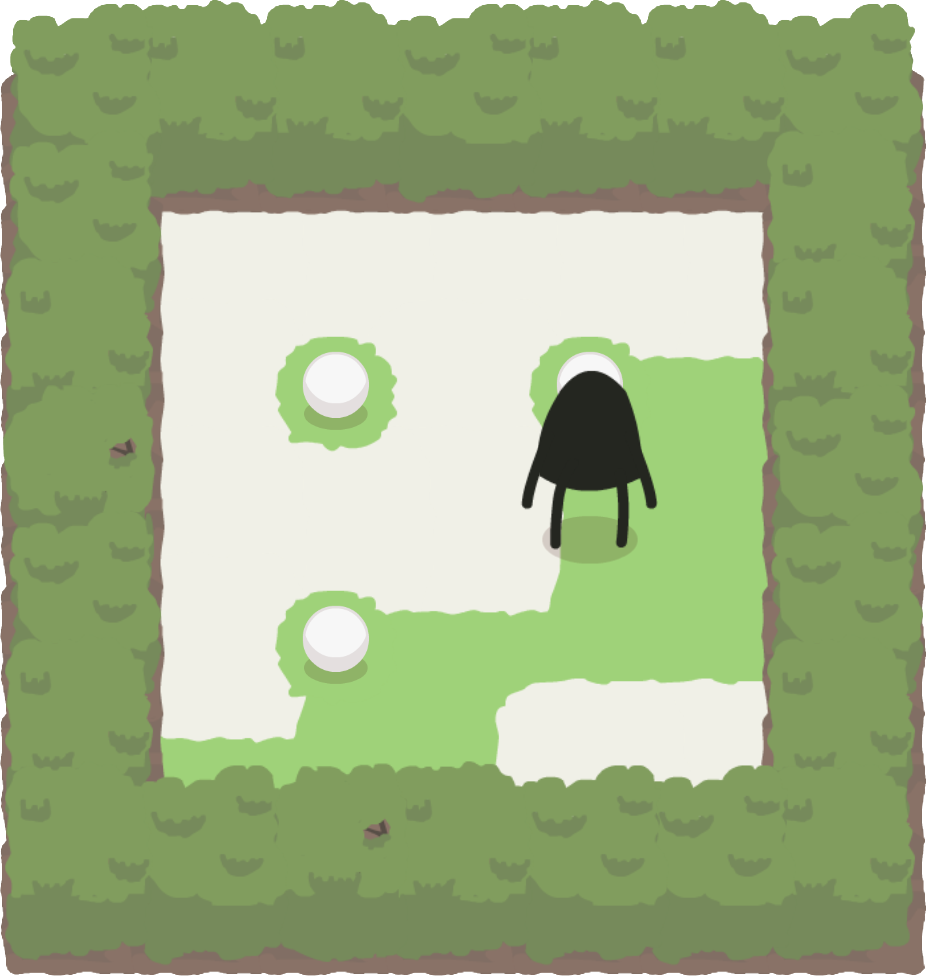
\includegraphics[width=\andyWidth\textwidth]{andy-basic-2.png} \quad
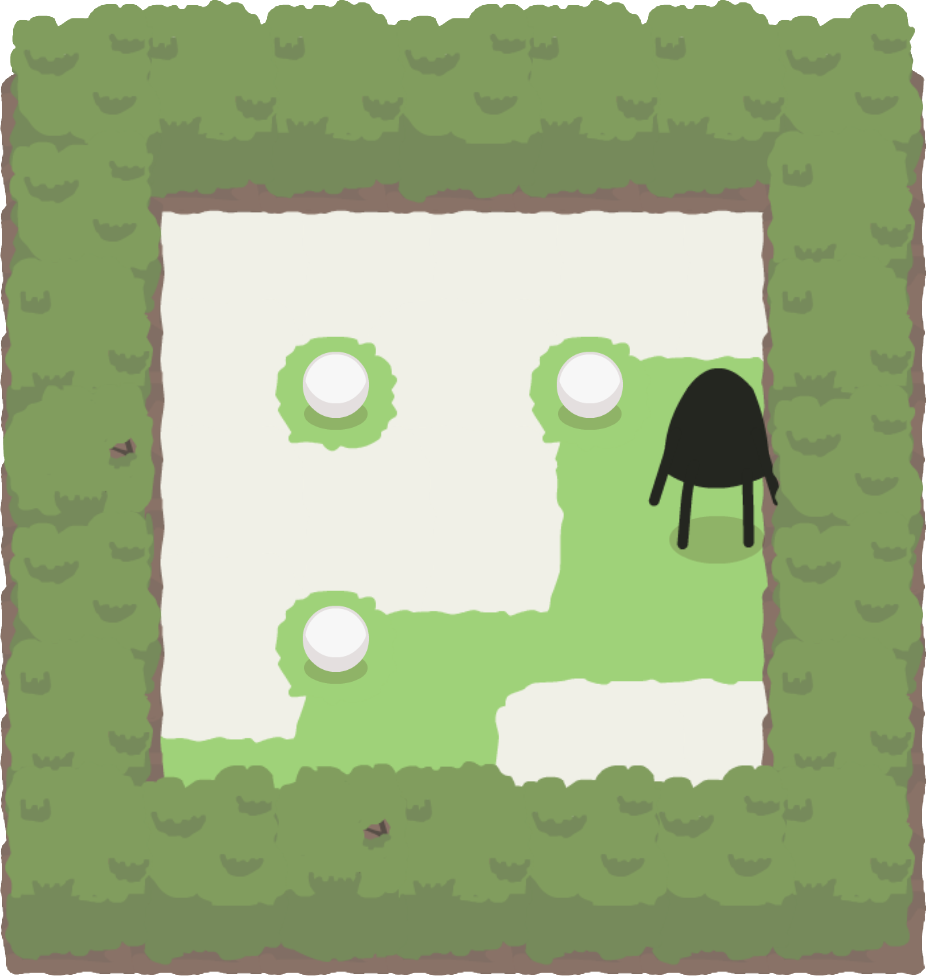
\includegraphics[width=\andyWidth\textwidth]{andy-basic-3.png} \quad
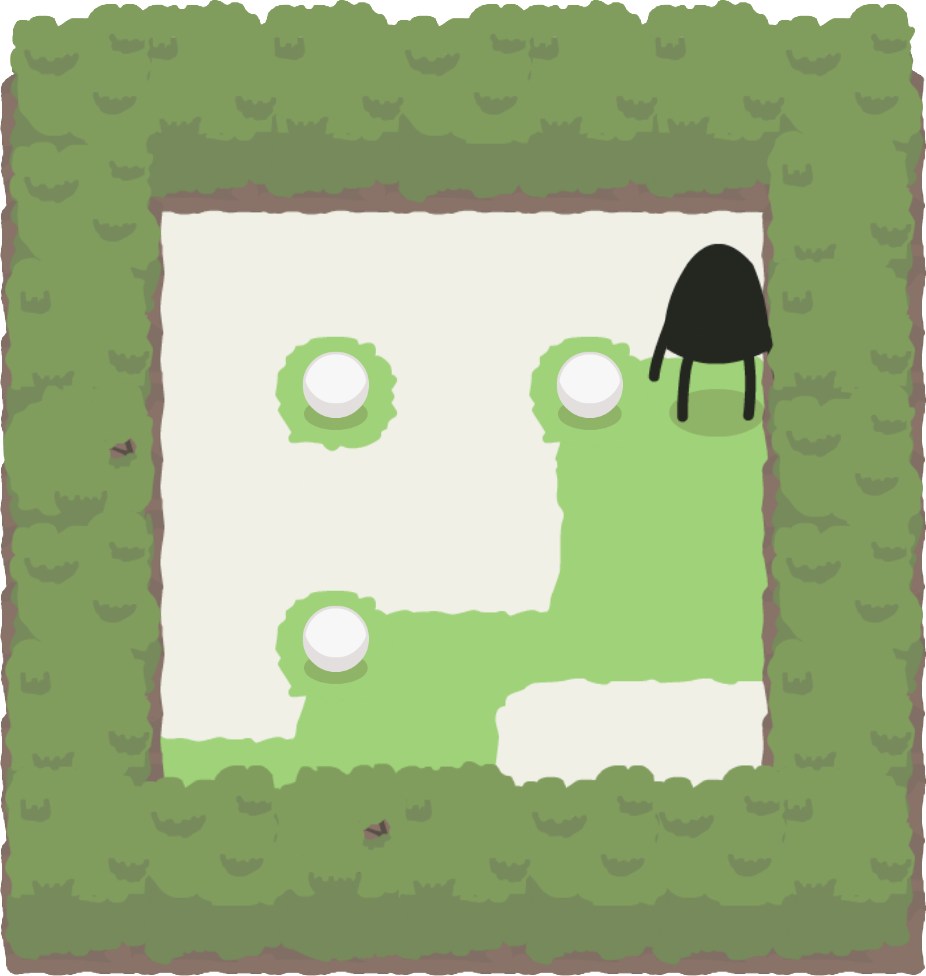
\includegraphics[width=\andyWidth\textwidth]{andy-basic-4.png}
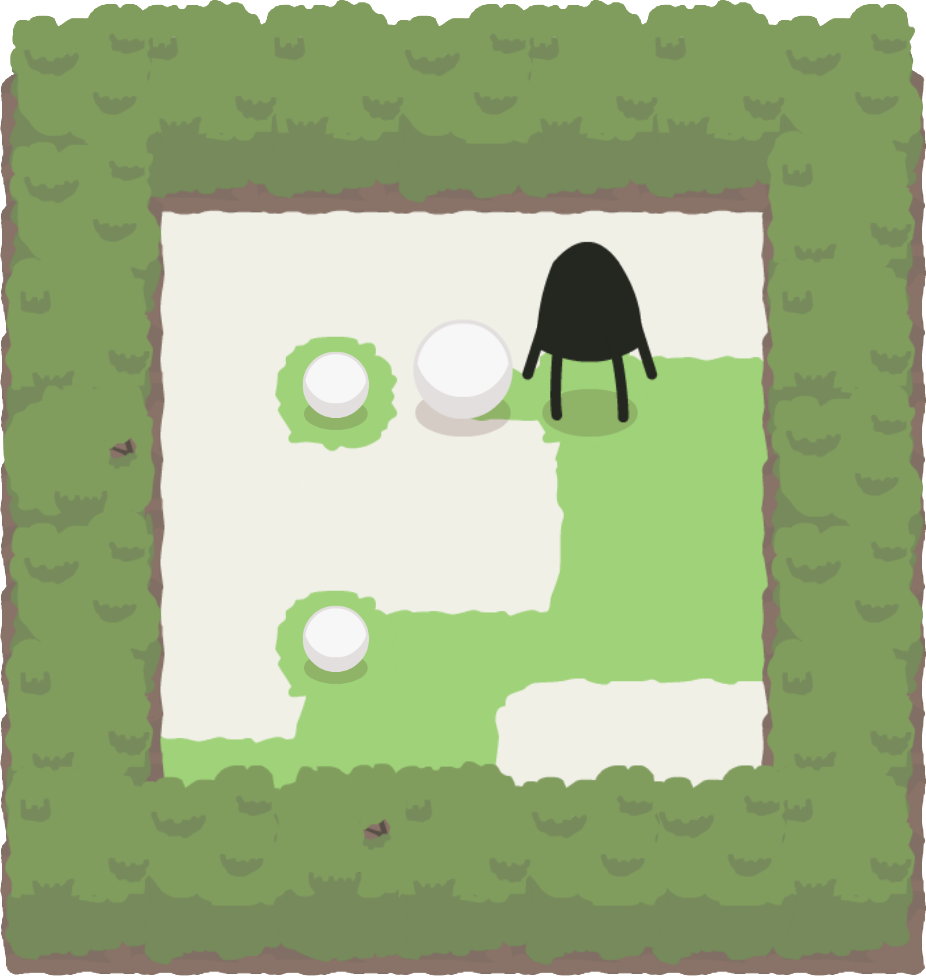
\includegraphics[width=\andyWidth\textwidth]{andy-basic-5.png} \quad
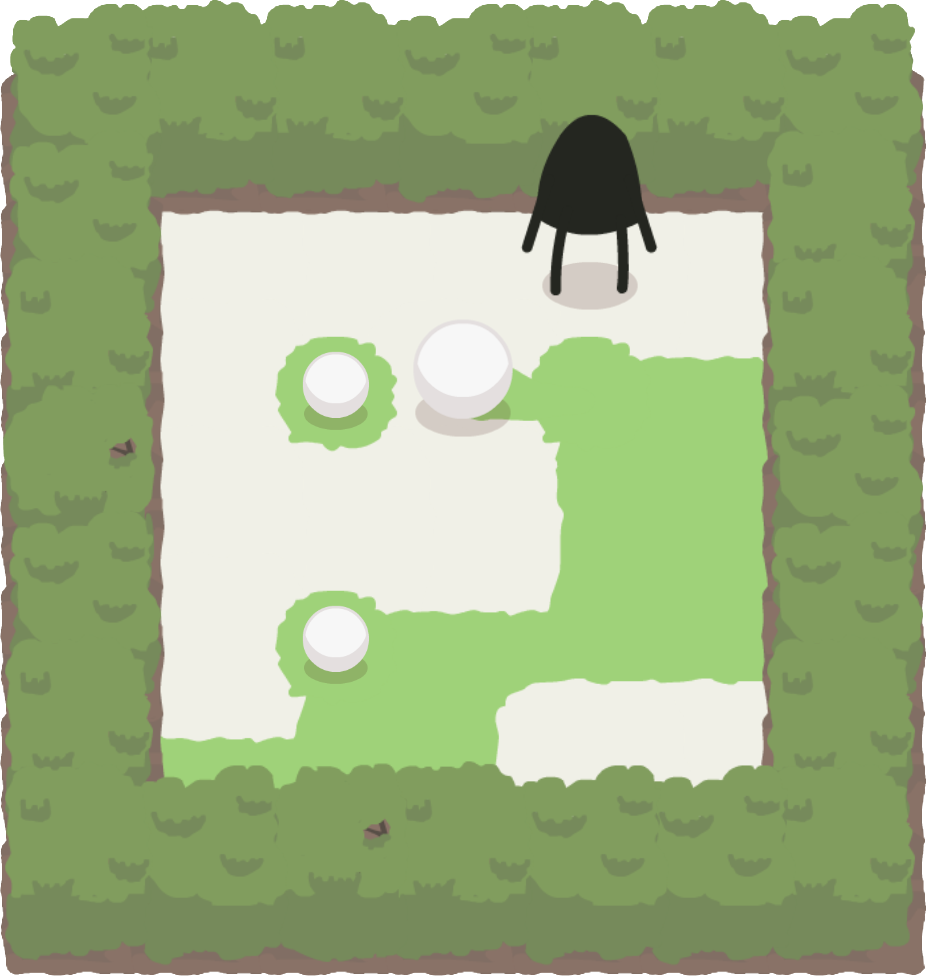
\includegraphics[width=\andyWidth\textwidth]{andy-basic-6.png} \quad
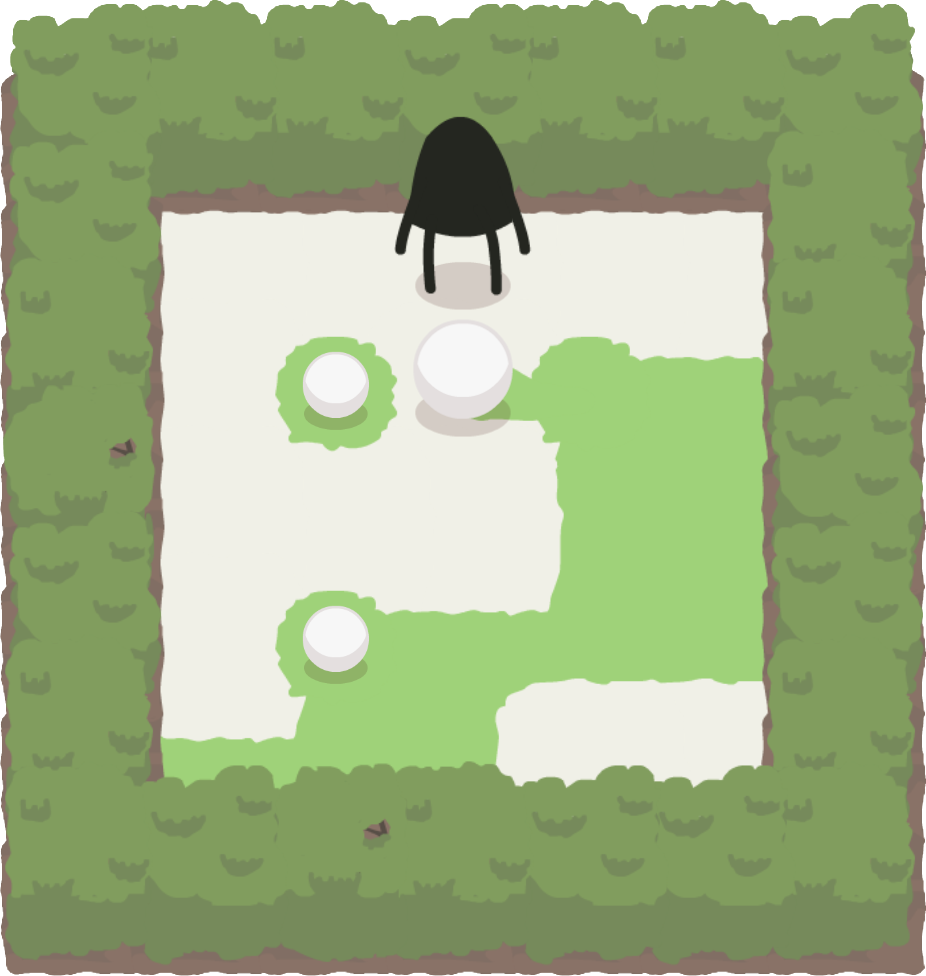
\includegraphics[width=\andyWidth\textwidth]{andy-basic-7.png} \quad
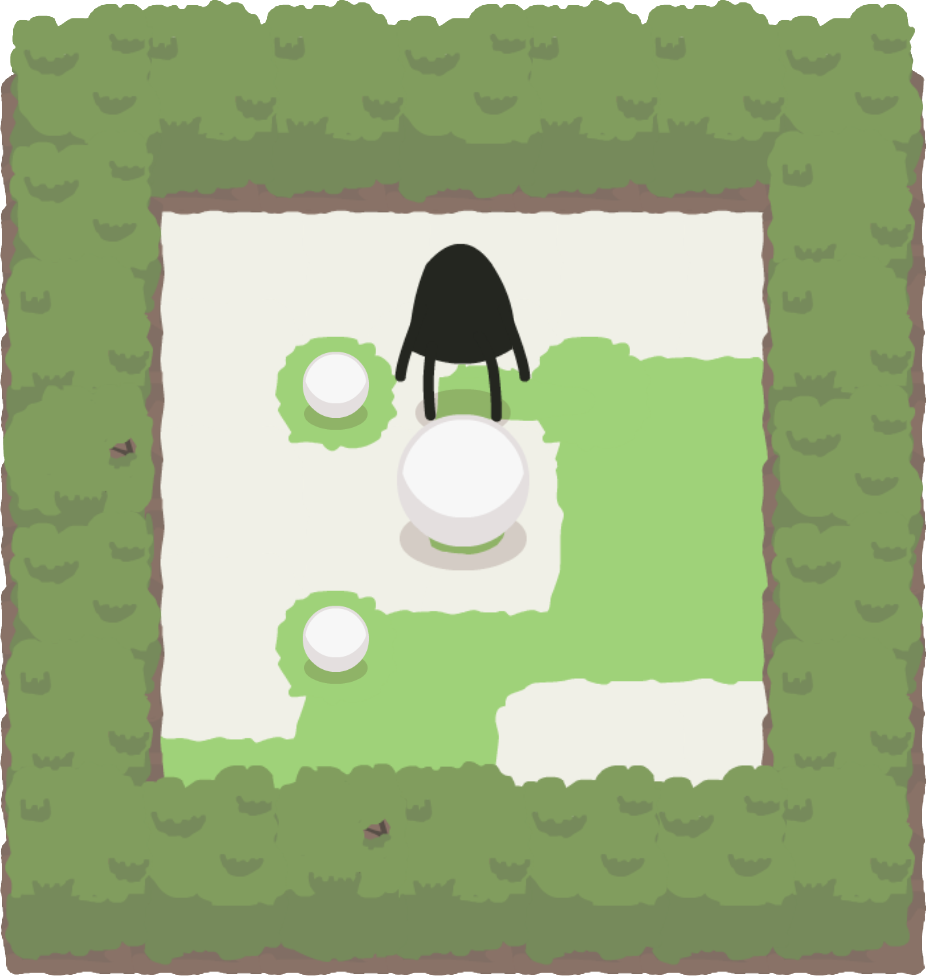
\includegraphics[width=\andyWidth\textwidth]{andy-basic-8.png}
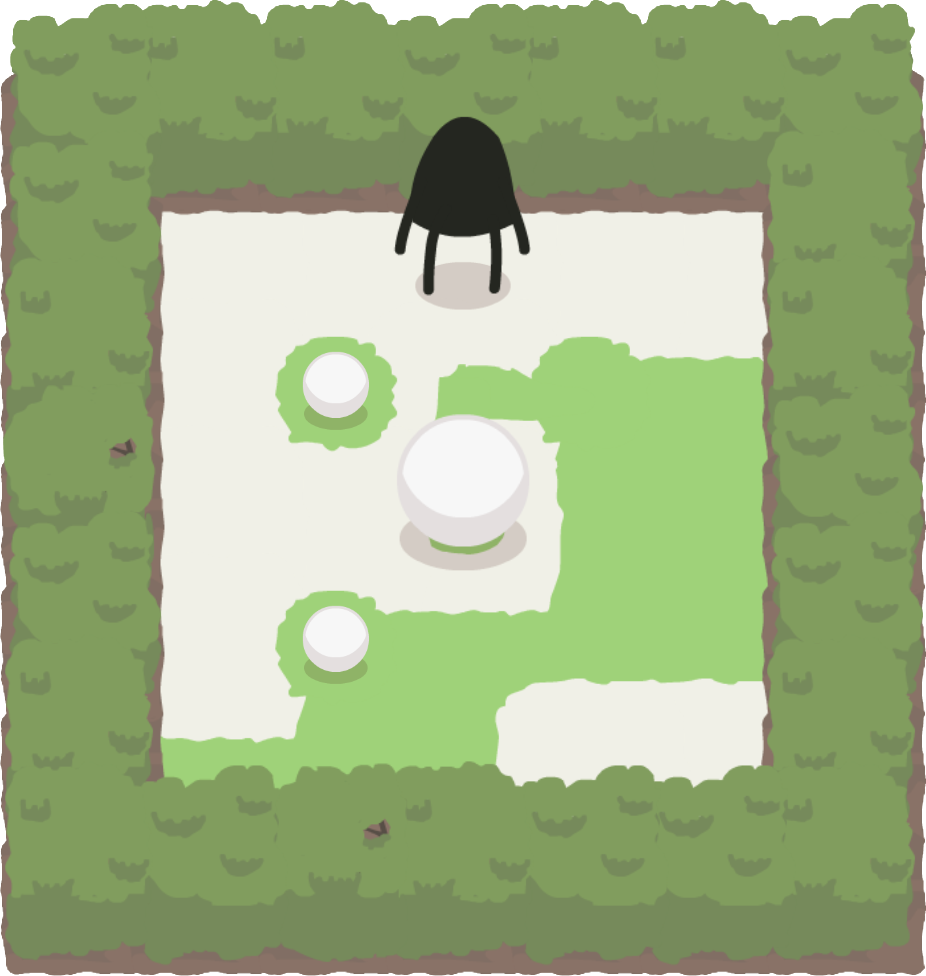
\includegraphics[width=\andyWidth\textwidth]{andy-basic-9.png} \quad
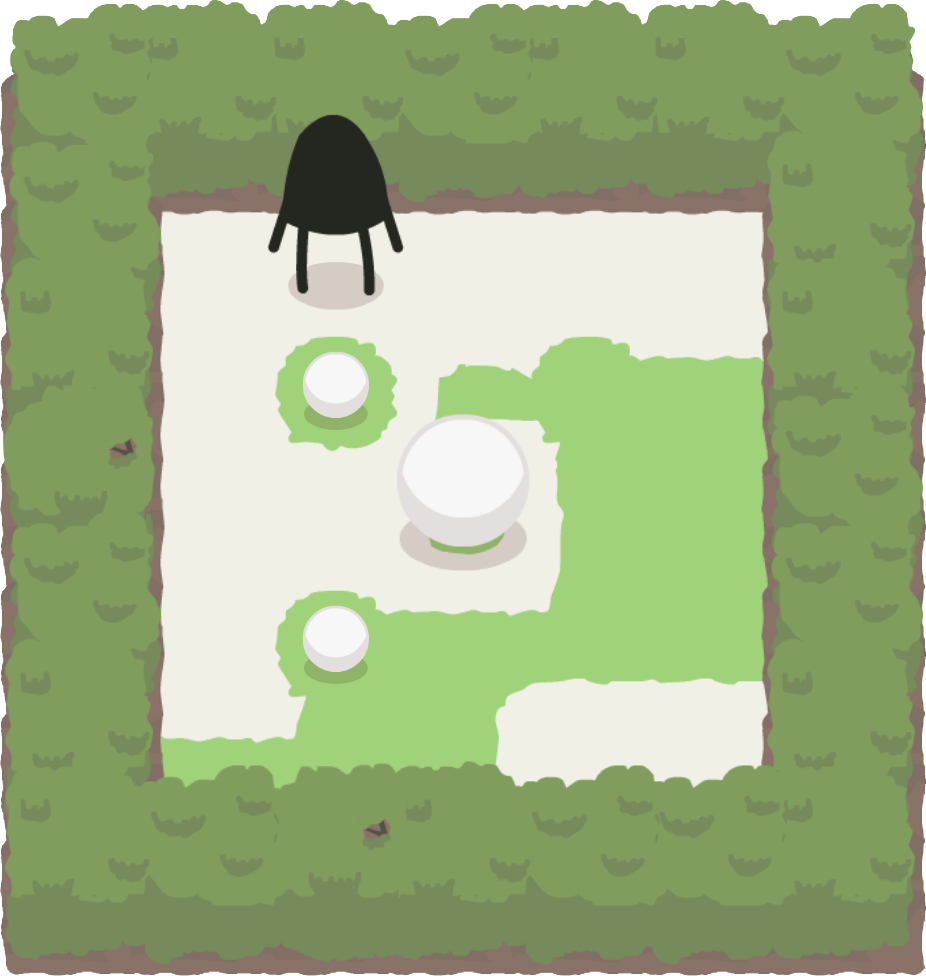
\includegraphics[width=\andyWidth\textwidth]{andy-basic-10.png} \quad
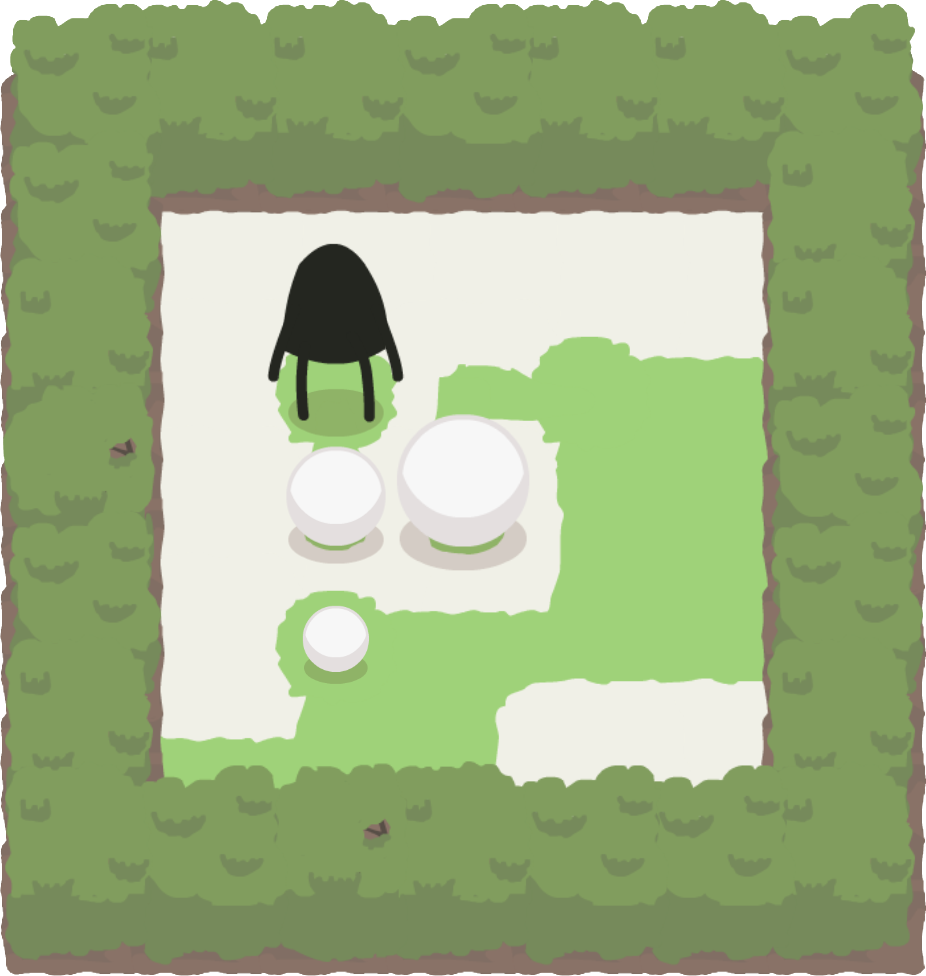
\includegraphics[width=\andyWidth\textwidth]{andy-basic-11.png} \quad
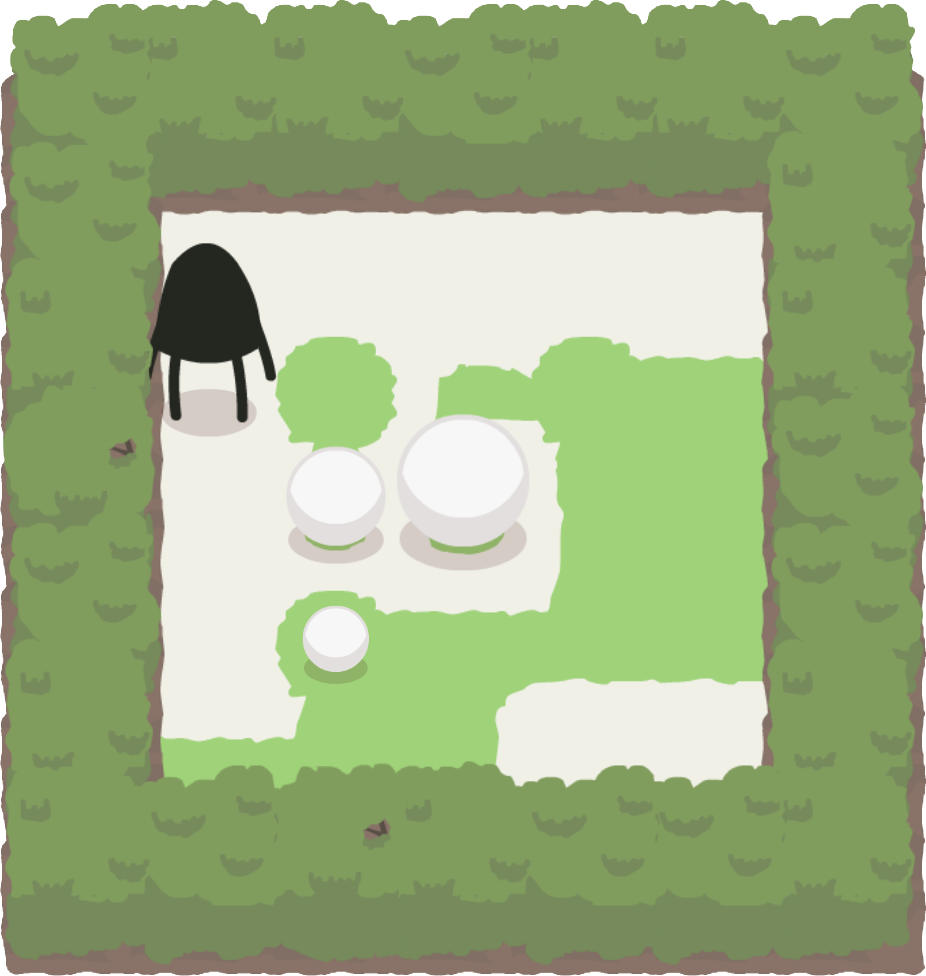
\includegraphics[width=\andyWidth\textwidth]{andy-basic-12.png}
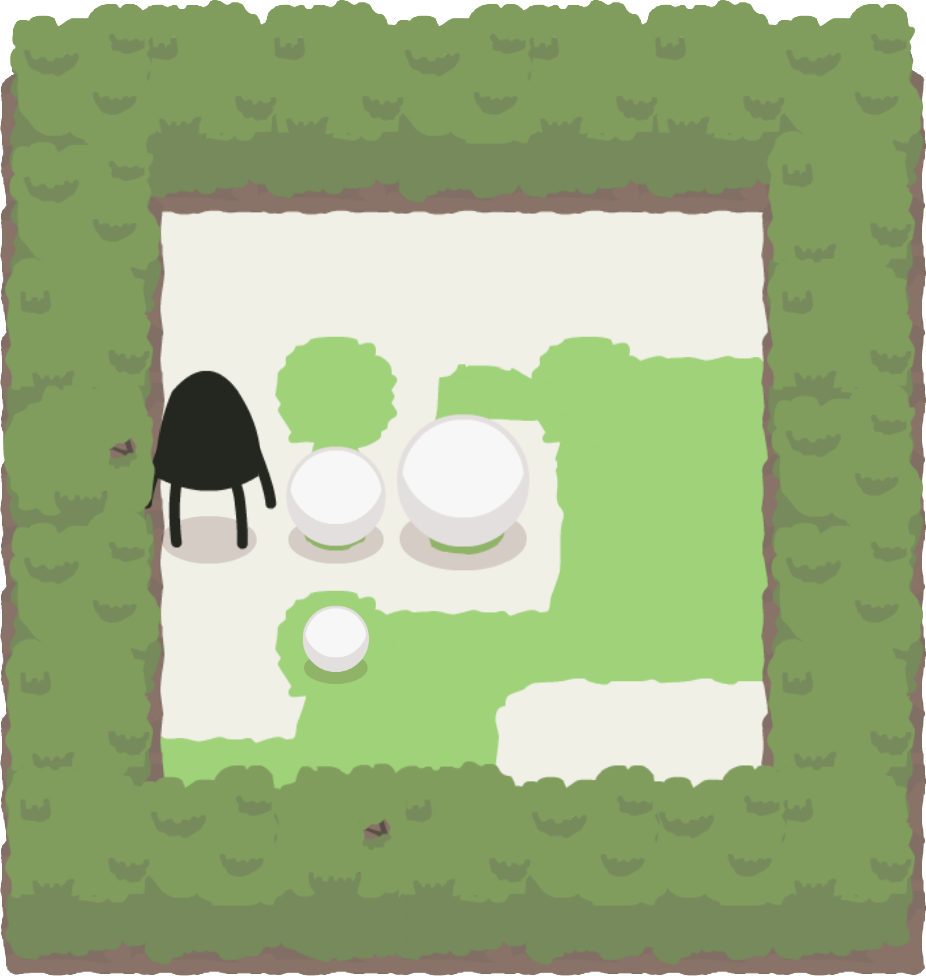
\includegraphics[width=\andyWidth\textwidth]{andy-basic-13.png} \quad
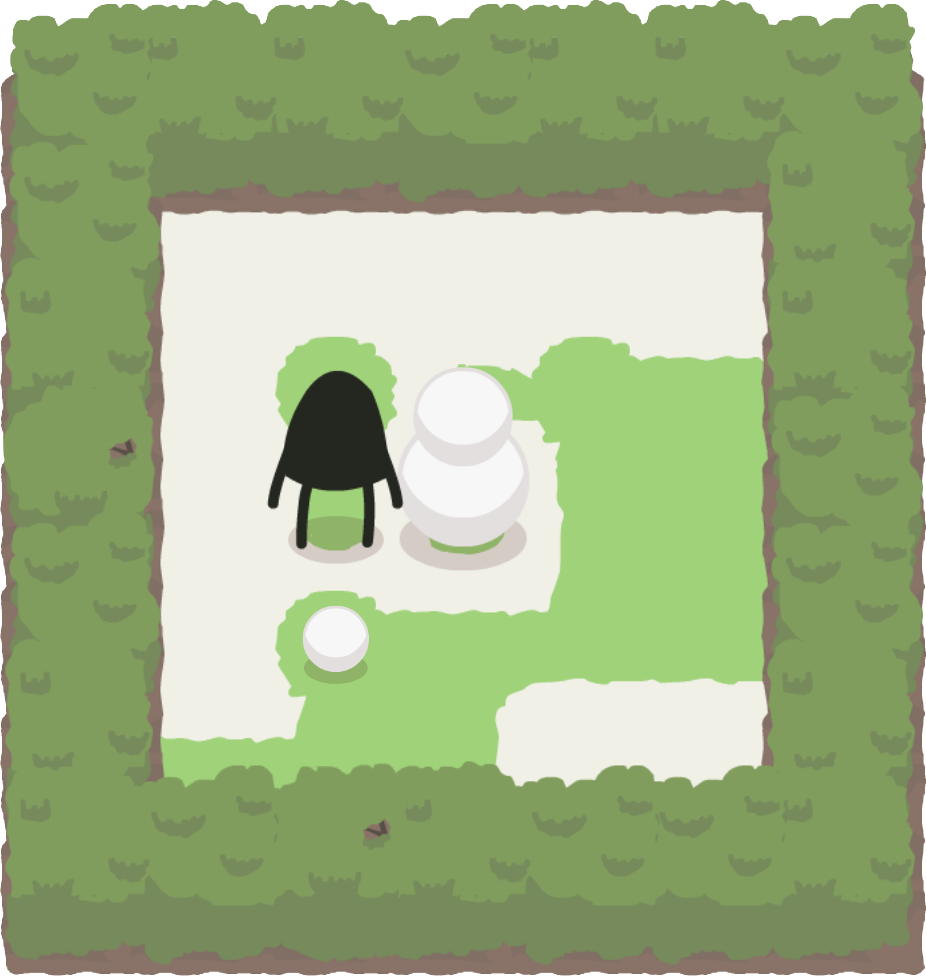
\includegraphics[width=\andyWidth\textwidth]{andy-basic-14.png} \quad
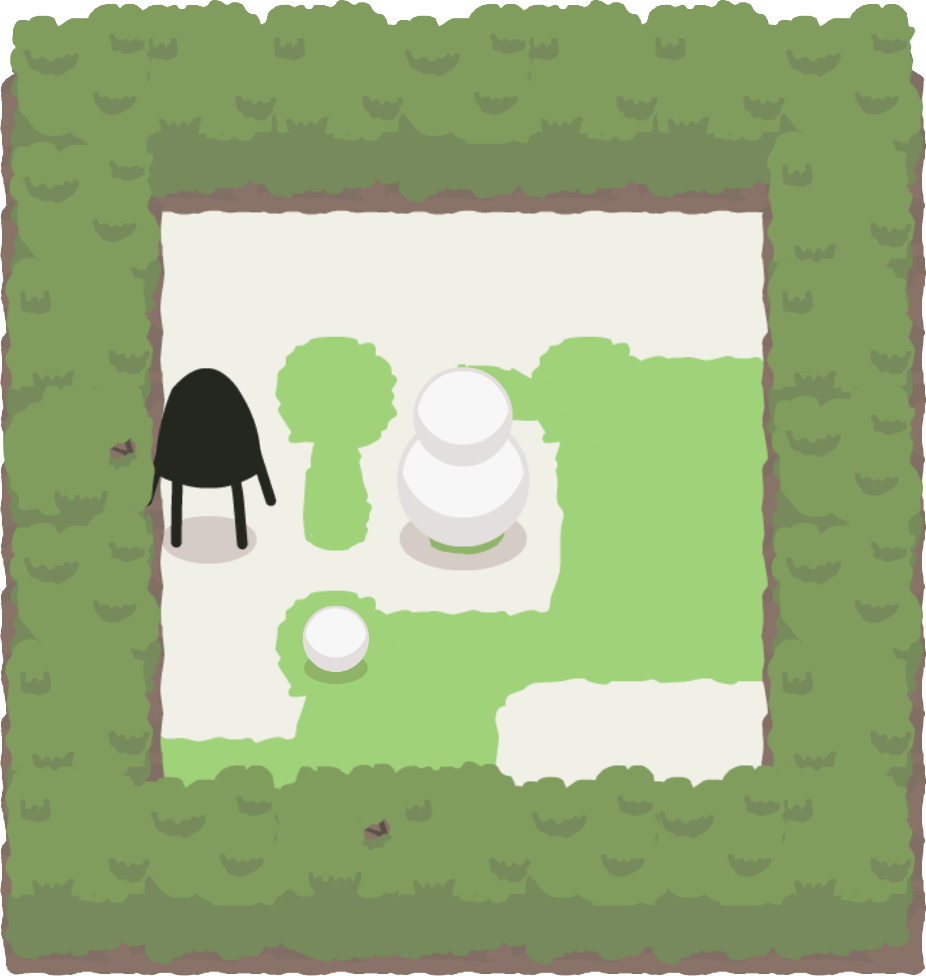
\includegraphics[width=\andyWidth\textwidth]{andy-basic-15.png} \quad
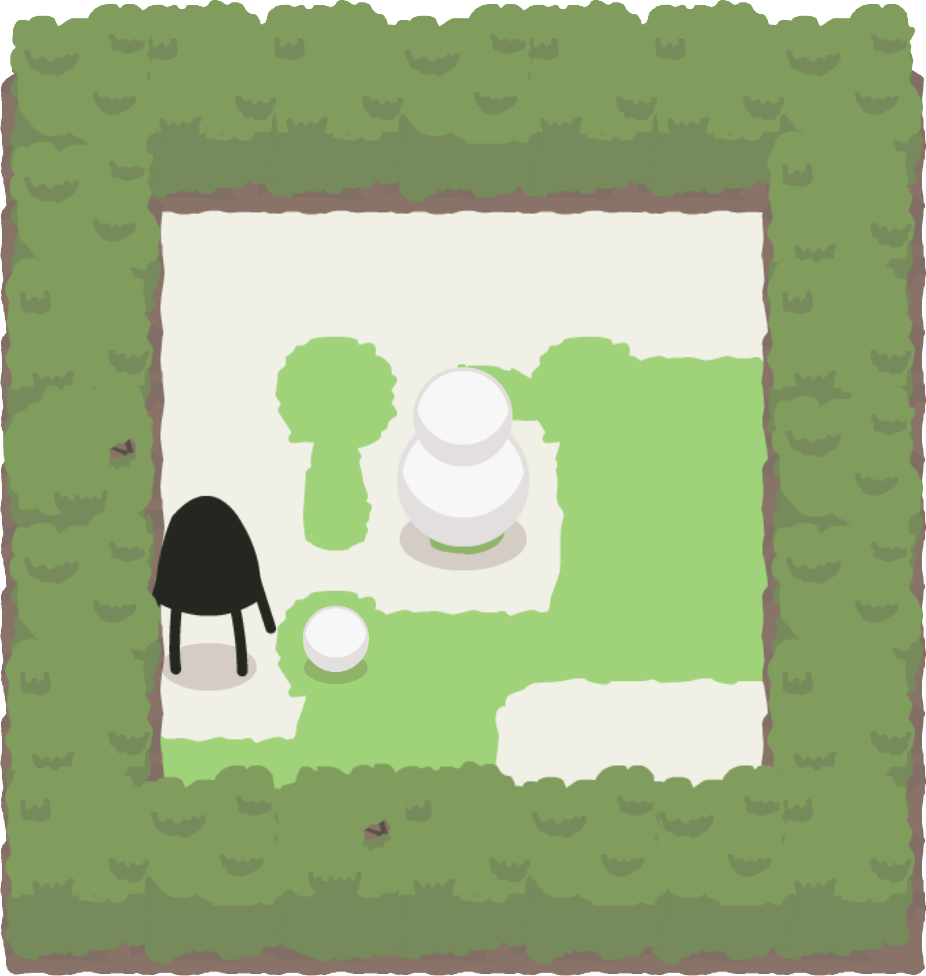
\includegraphics[width=\andyWidth\textwidth]{andy-basic-16.png}
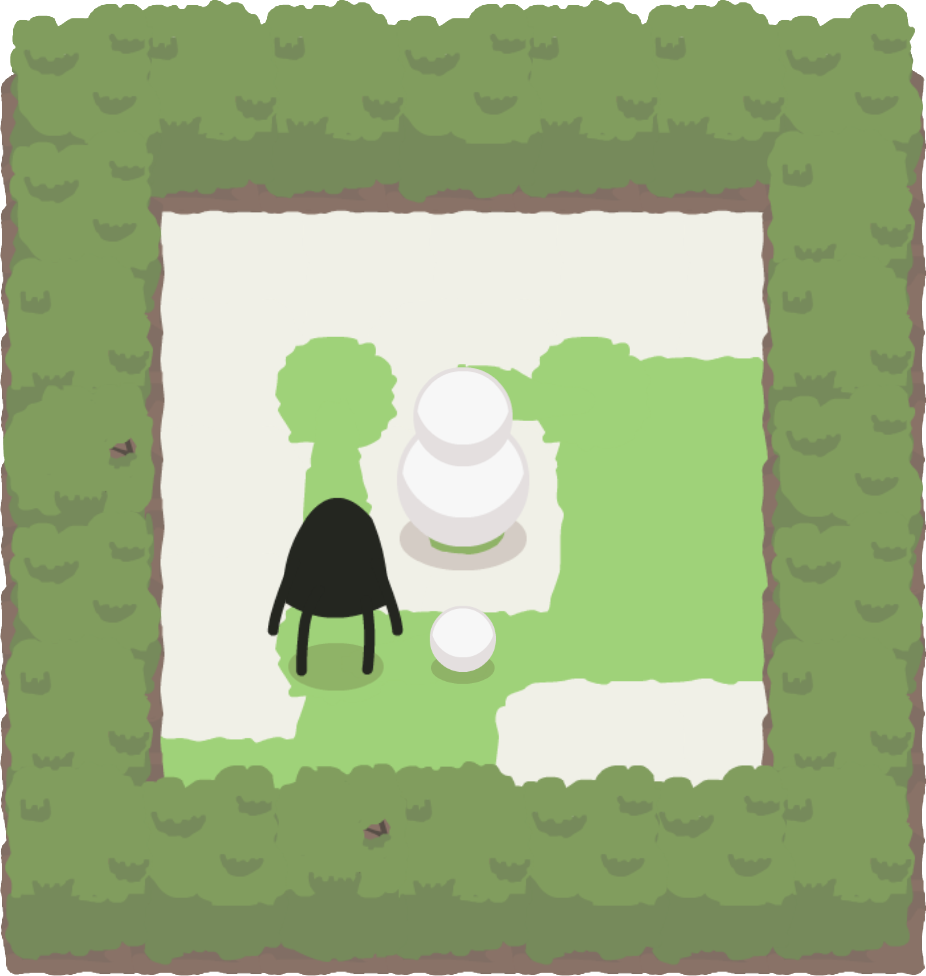
\includegraphics[width=\andyWidth\textwidth]{andy-basic-17.png} \quad
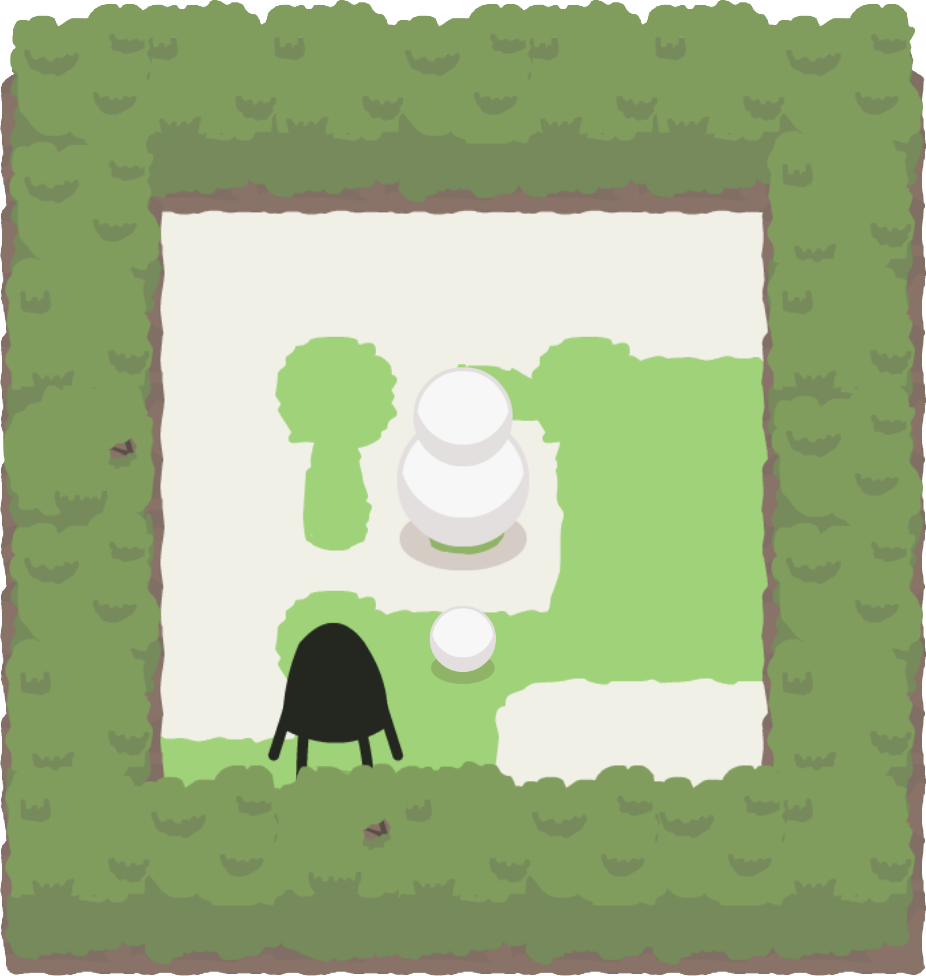
\includegraphics[width=\andyWidth\textwidth]{andy-basic-18.png} \quad
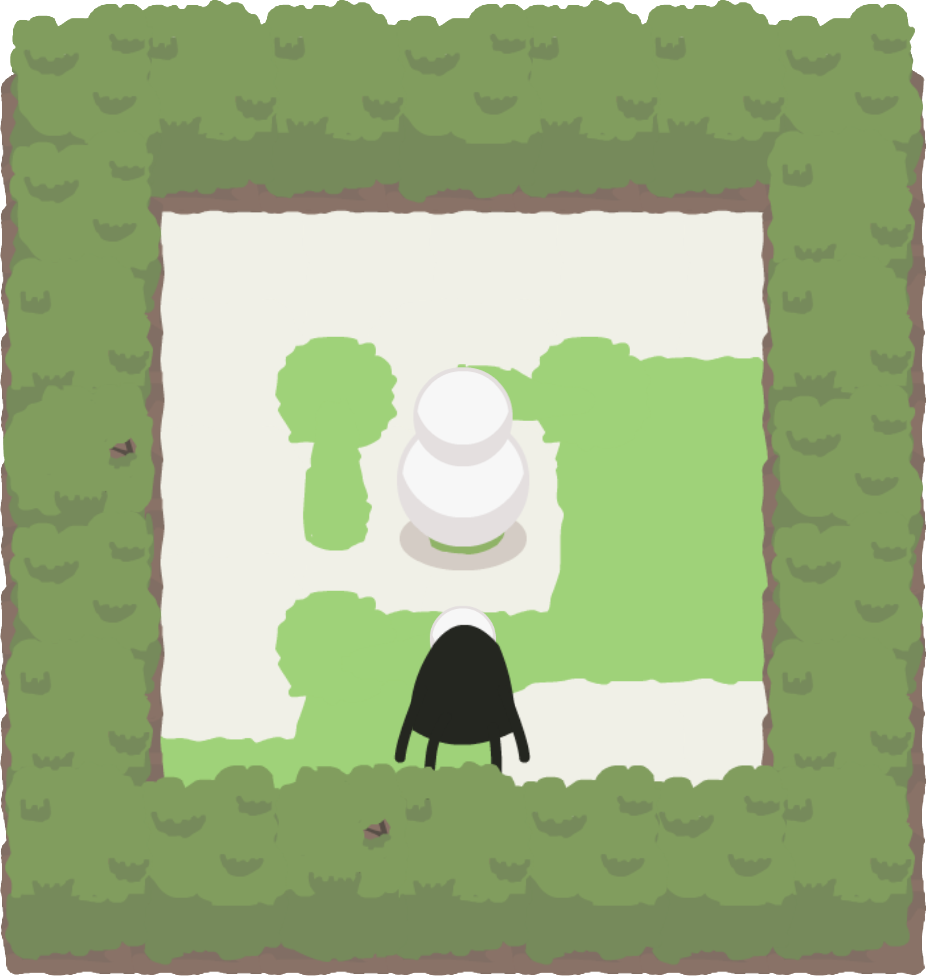
\includegraphics[width=\andyWidth\textwidth]{andy-basic-19.png} \quad
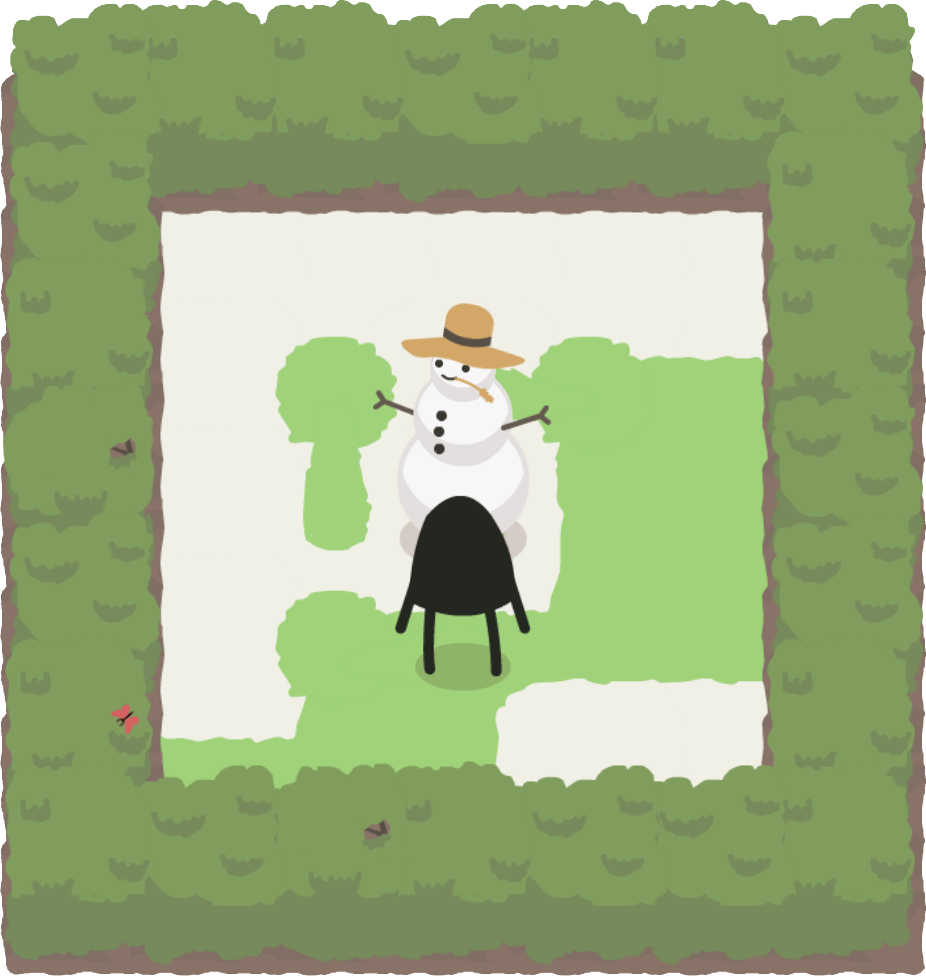
\includegraphics[width=\andyWidth\textwidth]{andy-basic-20.png}
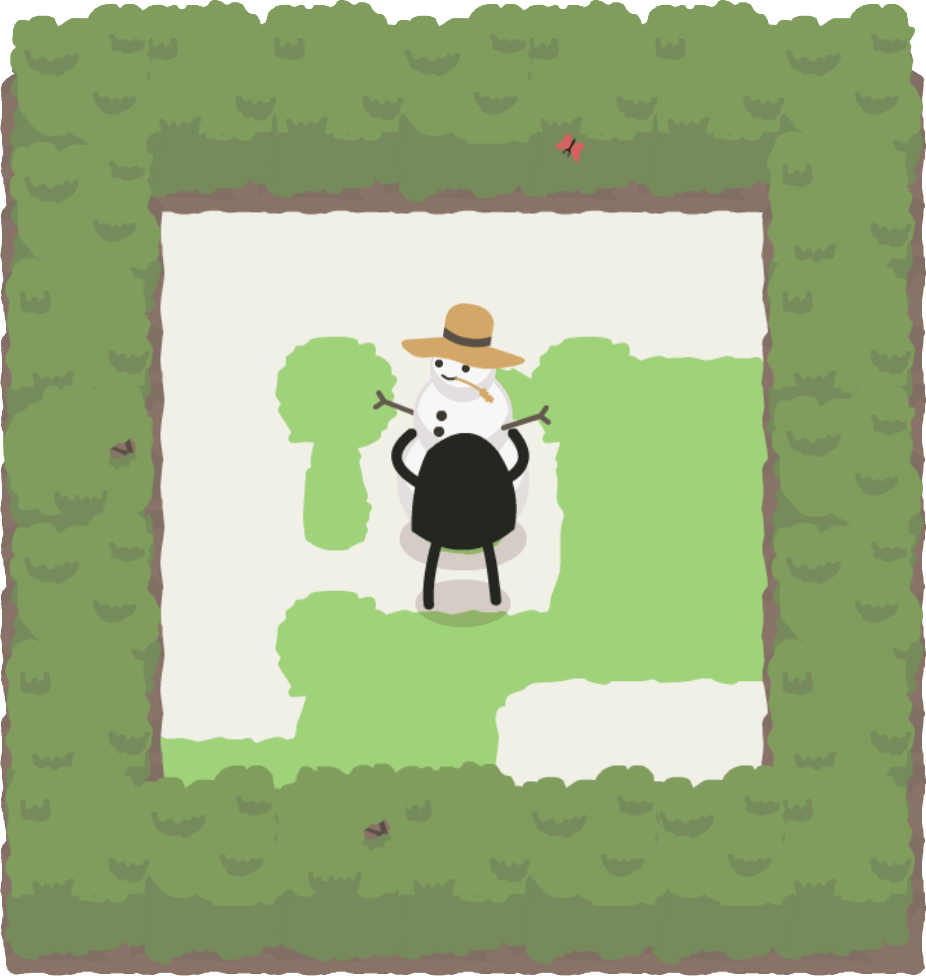
\includegraphics[width=\andyWidth\textwidth]{andy-basic-21.png}
\end{center}
\end{example}

\chapter{Design}
\section{Snowman editor}
The \emph{Snowman editor} (Figure~\ref{fig:gui} ) is a complete tool which facilitates the level design by allowing the user to create a new level, try it in-game and also find a solution. The tool has multiple solvers which use the SMT approach but also allows to generate PDDL problem instances which can be used externally with the desired planner.

\begin{figure}
    \begin{minipage}{0.5\textwidth}
    \centering
    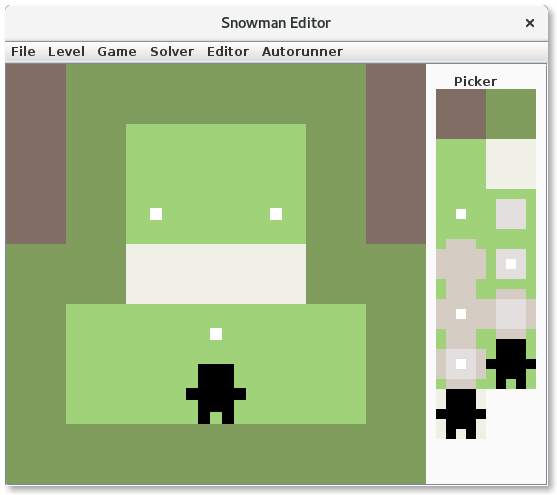
\includegraphics[width=0.8\textwidth]{gui-1.png}
    \end{minipage}
    \begin{minipage}{0.5\textwidth}
    \centering
    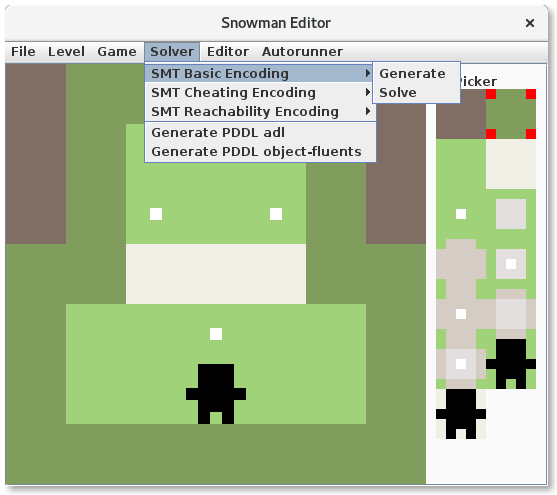
\includegraphics[width=0.8\textwidth]{gui-2.png}
    \end{minipage}
    \caption{\emph{Snowman Editor} with the level Sarah loaded. The tool is composed by a level representation (right), a tile type picker (right) and a menu bar (top) which allow to use all the tool functionalities.}
    \label{fig:gui}
\end{figure}

\section{PDDL Approach}
The PDDL approach aims to solve the \emph{Snowman problem} by using the PDDL standard Artificial Intelligence planning language. Because of the limitations with PDDL and its planers, two different approaches have been taken. 

\subsection{\emph{adl} approach}
The main idea behind the \emph{adl} approach is to associate a distinct object to each possible locations of the level at hand. But, the main problem with this approach is the number of action which because it is to large, makes the search impossible.

\subsection{object-fluents approach}
The \emph{object-fluents} approach aims to reduce the number of actions, but, in the current state of the art, there do not exist planners which supports this newer language subset.

\section{SMT Approach}
The SMT approach allows to find an optimal solution to the \emph{Snowman problem}. This is desired since the main objective of the project is to find undesired solutions, which usually are easier solutions that the wanted solution.

During the encoding development process three different encodings have been created since each one has its advantages an inconveniences. The theory used is Linear Integer Arithmetic since integer variables and linear arithmetic expressions are required.

\subsection{Basic encoding: The first SMT encoding}
A first approach to encode the \emph{Snowman problem} is to encode all possible actions a player can do in the game. Even though there are only four actions in the game (up, down, left, right)\footnote{The game is played using the keyboard arrows}, since they have different effects, these actions can be split into two categories: character movement actions and ball movement actions.

This way, this first encoding encodes four actions for the character movement actions and four actions for the ball movement actions, but for each ball. To perform a ball movement action, first the player has to travel next to the ball using the character movements actions.

The preliminary result however, showed that this first encoding was not able to solve many levels in a reasonable time.

\subsection{Cheating encoding}
This encoding is based on the previous encoding, but it removes the character movement actions allowing the character to teleport anywhere on the map as long as is not occupied. This can be seen as cheating, as a ball can block a path to a candidate ball movement action.


\subsection{Reachability encoding}
The \emph{Reachability encoding} is based on the previous \emph{Cheating encoding}, but it introduces a new reachability precondition. These preconditions ensure that there is a path from the position of the character when doing a ball movement action to the position of the character to perform the next ball movement action. 

\subsubsection{Reachability precondition}
The reachability precondition encodes an \emph{s-t-reachability} problem extending the \emph{Topological Sort with Indices} described in the article \emph{SAT modulo graphs: Acyclicity}. Is important to remark that in contrast to the article, this extension must deal with non-static graphs in the sense that it is not know, when the the encoding is being build, which will be the source and which will be the target of the s-t-reachability problem. Neither is not known which positions will be occupied. Therefore, we believe that this is a remarkable contribution of this project.

\end{document}
